\chapter{Investigation and Evaluation}
\label{ch:evaluation}

\section{Experimental Investigation}

\subsection{Evaluation questions and protocols}

The investigation tests three hypotheses: (H1) temporal models can learn useful
physical-PAD evidence; (H2) strong source-domain performance will decline under a
shift from physical spoofs to high-quality digital manipulation; and (H3)
manipulation-specific specialists with a learned router can outperform one
universal frame detector on a controlled in-domain split.

The physical/deepfake transfer study uses LCC-FASD, Celeb-DF-v2, and Asian-Fakes.
Two saved protocols are compared for each of $G^2V^2$former and GD-FAS: training
on LCC-FASD, and then fine-tuning the resulting model on Celeb-DF-v2. All three
datasets are evaluated after each stage. This is a demanding domain shift because
physical replay/print cues and digital synthesis cues are not interchangeable.
Celeb-DF-v2 itself was constructed to reduce the obvious artefacts of older
deepfake data \cite{li2020celebdf}.

The Xception study uses FaceForensics++ C23. Validation is group-disjoint from
training at the source-video group level. The universal detector sees original
and all five fake methods. Each specialist sees original versus one method. Two
legacy routers---a CNN head and XGBoost---predict one of six original/method
classes from embeddings and then dispatch to a specialist or apply the original
fallback. This protocol answers an in-domain routing question only; it is not an
unseen-generator or production-liveness evaluation.

\subsection{Metrics}

Let bona fide be the negative class and attack/fake the positive class. Accuracy
can be inflated by class imbalance, so balanced accuracy and class-conditional
rates are reported. For PAD experiments,

\begin{align}
\mathrm{APCER} &= \frac{\text{attacks classified as bona fide}}{\text{all attacks}},\\
\mathrm{BPCER} &= \frac{\text{bona fide classified as attack}}{\text{all bona fide}},\\
\mathrm{HTER} &= \frac{\mathrm{APCER}+\mathrm{BPCER}}{2}.
\end{align}

ROC-AUC measures ranking across thresholds; average precision (AP) is informative
under fake-heavy class balance. None of these, by itself, establishes calibrated
probability, robustness to injection, or a financially acceptable operating
point. ISO/IEC 30107-3 reporting should be followed for a formal PAD evaluation
\cite{iso30107}.

\section{Performance Evaluation}

\subsection{Temporal and domain-generalisation results}

\Cref{tab:transfer-results} gives the results reproduced across the current plan
and inspected experiment artefacts. Values are percentages. The source-only
$G^2V^2$former result demonstrates useful LCC-FASD discrimination but transfers
poorly to Celeb-DF-v2. GD-FAS is exceptionally strong on its source data yet also
falls to near-chance target behaviour. Fine-tuning on Celeb-DF-v2 improves target
and Asian-Fakes results for both models, but the target HTER remains high and
source performance decreases.

\begin{table}[H]
\centering
\caption{Common-protocol cross-domain results (\%). Lower HTER and higher AUC are
better.}
\label{tab:transfer-results}
\small
\begin{tabular}{@{}llrrrrrr@{}}
\toprule
& & \multicolumn{2}{c}{LCC-FASD} & \multicolumn{2}{c}{Celeb-DF-v2} &
\multicolumn{2}{c}{Asian-Fakes}\\
\cmidrule(lr){3-4}\cmidrule(lr){5-6}\cmidrule(l){7-8}
Model & Training stage & HTER & AUC & HTER & AUC & HTER & AUC \\
\midrule
$G^2V^2$former & LCC-FASD & 22.38 & 80.71 & 59.71 & 37.14 & 50.13 & 49.82 \\
$G^2V^2$former & $+$ Celeb-DF-v2 & 33.50 & 65.14 & 43.32 & 57.22 & 49.13 & 50.33 \\
GD-FAS & LCC-FASD & \textbf{4.55} & \textbf{99.69} & 52.99 & 50.49 & 48.33 & 52.98 \\
GD-FAS & $+$ Celeb-DF-v2 & 7.07 & 99.16 & \textbf{41.04} & \textbf{64.35} & \textbf{44.58} & \textbf{57.94} \\
\bottomrule
\end{tabular}
\end{table}

These results do not show that temporal information is unhelpful. They show that
temporal modelling does not remove the need for representative domains and
generator diversity. A model may learn the motion of print/replay attacks while
missing temporally plausible face swaps. Conversely, GD-FAS's source result does
not prove digital manipulation generalisation. The appropriate conclusion is
that attack taxonomy, training domains, and evaluation domains must be reported
together.

An earlier ROSE-Youtu MobileNetV3 temporal experiment recorded 98.46\% accuracy,
99.88\% AUC, 1.39\% EER, and 1.36\% HTER. It is retained as evidence that the
lightweight temporal approach can perform strongly on the earlier physical-PAD
protocol. It must not be attributed to the current 24-frame exported checkpoint
until its training provenance is reconciled, and it does not establish deepfake
or injection robustness.

The inspected $G^2V^2$former latency pilot used five runs on an NVIDIA T4 and
reported a mean of 1,315.45 ms per video end-to-end, of which 134.56 ms was model
inference. The small run count and cloud GPU environment make this a diagnostic,
not a production latency guarantee. The difference between total and model time
also shows that face/landmark preprocessing and data handling deserve optimisation.

\draftnote{The latest prior PDF mentions a best $G^2V^2$former HTER of 21.71\%,
whereas the common-protocol table and inspected artefacts contain 22.38\% (and
another checkpoint value of 24.07\%). Select the final checkpoint by a declared
rule and regenerate the table before submission.}

\subsection{Universal and routed Xception results}

\Cref{tab:routing-overall} compares the three saved FaceForensics++ validation
results. The routed CNN improves every reported aggregate metric relative to the
universal detector, including real-class accuracy. XGBoost also improves balanced
accuracy, ROC-AUC, and AP, but underperforms the CNN router.

\begin{table}[H]
\centering
\caption{Current six-way in-domain routing results on the group-disjoint
FaceForensics++ validation set (\%).}
\label{tab:routing-overall}
\small
\begin{tabular}{@{}lrrrrrr@{}}
\toprule
System & Accuracy & Balanced acc. & ROC-AUC & AP & Real acc. & Fake acc. \\
\midrule
Universal Xception & 81.83 & 76.44 & 86.32 & 96.62 & 68.37 & 84.52 \\
CNN-routed specialists & \textbf{84.44} & \textbf{84.51} & \textbf{91.68} & \textbf{98.22} & \textbf{84.62} & \textbf{84.40} \\
XGBoost-routed specialists & 83.49 & 82.39 & 88.73 & 97.73 & 80.73 & 84.05 \\
\bottomrule
\end{tabular}
\end{table}

\begin{figure}[H]
\centering
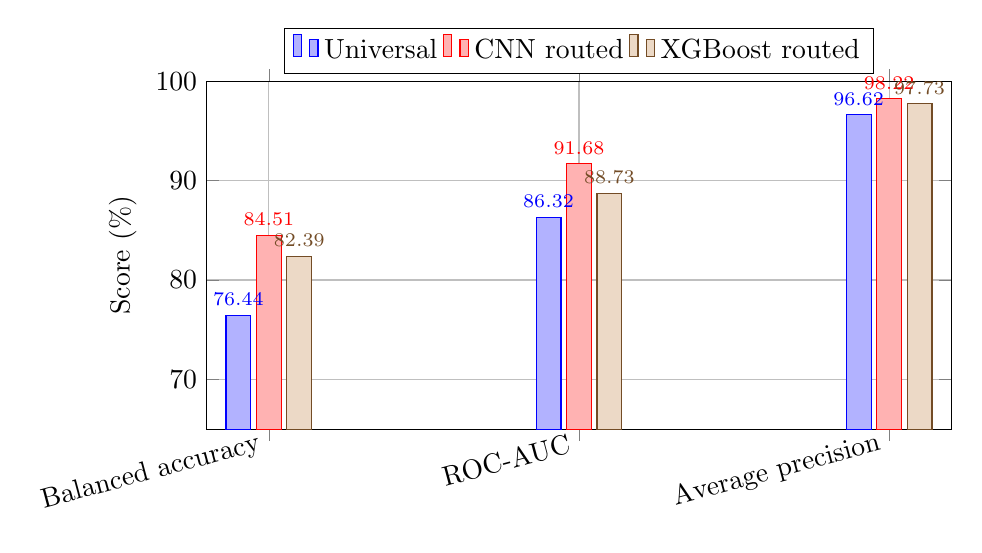
\begin{tikzpicture}
\begin{axis}[
  ybar, bar width=9pt, width=0.91\textwidth, height=60mm,
  ymin=65,ymax=100, ylabel={Score (\%)},
  symbolic x coords={Balanced accuracy,ROC-AUC,Average precision},
  xtick=data, x tick label style={rotate=15,anchor=east},
  legend style={at={(0.5,1.02)},anchor=south,legend columns=3},
  nodes near coords, nodes near coords style={font=\scriptsize},
  grid=major
]
\addplot coordinates {(Balanced accuracy,76.44) (ROC-AUC,86.32) (Average precision,96.62)};
\addplot coordinates {(Balanced accuracy,84.51) (ROC-AUC,91.68) (Average precision,98.22)};
\addplot coordinates {(Balanced accuracy,82.39) (ROC-AUC,88.73) (Average precision,97.73)};
\legend{Universal,CNN routed,XGBoost routed}
\end{axis}
\end{tikzpicture}
\caption{Aggregate routing comparison. The plot visualises the current six-way
artefact and must not be relabelled as the intended five-expert rerun.}
\label{fig:routing-bars}
\end{figure}

Per-method balanced accuracy in \Cref{tab:routing-method} explains why the idea
is promising. Every specialist outperforms the universal detector for its method,
and routing recovers part, but not all, of that oracle-like advantage. Router
mistakes therefore remain a measurable bottleneck. NeuralTextures is the hardest
of the five classes for the specialist and routed systems.

\begin{table}[H]
\centering
\setlength{\tabcolsep}{10pt}
\caption{Per-manipulation balanced accuracy of specialist, universal, and current
routed CNN systems (\%).}
\label{tab:routing-method}
\begin{tabular}{@{}lrrr@{}}
\toprule
Manipulation & Matched specialist & Universal & Routed CNN \\
\midrule
Deepfakes & 94.86 & 79.81 & 88.62 \\
Face2Face & 92.36 & 78.47 & 85.20 \\
FaceShifter & 93.24 & 75.70 & 87.64 \\
FaceSwap & 90.37 & 75.58 & 84.98 \\
NeuralTextures & 80.28 & 72.66 & 76.11 \\
\bottomrule
\end{tabular}
\end{table}

The result supports a narrow conclusion: under the saved group-disjoint,
in-domain FF++ protocol, method-conditioned specialist selection improves a
universal Xception baseline. It does not demonstrate robustness to unseen
generators, external datasets, recapture, injection, video-level aggregation, or
deployment demographics. It also incurs an expert-training and storage cost that
must be compared with stronger universal or multi-task baselines.

\subsection{Assessment against objectives}

\begin{table}[H]
\centering
\caption{Objective-level evaluation status.}
\label{tab:objective-status}
\begin{tabularx}{\textwidth}{@{}p{38mm}p{24mm}Y@{}}
\toprule
Objective & Status & Evidence-based assessment \\
\midrule
Mobile temporal prototype & Partial success & Integrated 24-frame local path;
checkpoint/training provenance and device profiling remain. \\
Temporal deepfake transfer & Investigated & $G^2V^2$former results expose severe
domain shift; not yet operationally adequate. \\
Domain-generalised comparison & Investigated & GD-FAS strong in-domain, limited
cross-domain; fine-tuning improves target but remains weak. \\
Specialist routing & Promising, incomplete & Current six-way routing outperforms
universal baseline; intended five-expert best-model formulation requires rerun. \\
Layered end-to-end system & Not completed & Mobile and API artefacts exist
separately; fusion, escalation, review, and IAD are target design. \\
Fairness, privacy, and security validation & Not completed & Risks and requirements are
documented; demographic, field, red-team, and governance evaluation remain. \\
\bottomrule
\end{tabularx}
\end{table}

\section{Deviations and Design Revisions}

The main deviations are substantive and should remain visible in the final report:

\begin{enumerate}
  \item The planned three-tier system was narrowed to an integrated mobile first
        stage and separately tested server candidates; no reviewer interface was
        completed.
  \item The temporal MobileNet training code uses 10-frame clips in one path,
        whereas export/inference/application code uses 24; the final artefact
        cannot inherit earlier metrics without provenance evidence.
  \item $G^2V^2$former checkpoint metrics differ between the latest PDF and saved
        artefacts and require one reproducible final evaluation.
  \item Strong physical-PAD performance did not transfer to digital deepfakes,
        motivating GD-FAS comparison and manipulation-specific Xception work.
  \item The routing notebook added an original class, although the intended
        meta-router only selects among five specialists. Its useful six-way result
        is reported honestly, and the corrected five-way experiment is future work.
  \item Capture-channel attacks became an explicit system concern. Media analysis
        alone is no longer represented as sufficient protection from injection.
\end{enumerate}

These revisions improve the report's validity: they separate demonstrated
evidence from architecture intent and convert unresolved contradictions into
testable follow-up work.
